\def\xxactivite{Cours}

\def\xxauteur{P. Bessonnat -- Xavier Pessoles}
\fichefalse \proftrue \tdfalse \courstrue

\def\xxnumchapitre{Chapitre 11 \vspace{.2cm}}

\def\xxchapitre{Introduction aux graphes}

\def\xxcompetences{%
\textsl{%
\textbf{Savoirs et compétences :}\\
\begin{itemize}[label=\ding{112},font=\color{bleuxp}] 
\item Vocabulaire des graphes : graphe orienté, graphe non orienté. Sommet (ou nœud); arc, arête. Boucle. Degré (entrant et sortant). Chemin d’un sommet à un autre. Cycle. Connexité dans les graphes non orientés.
\item Notations : graphe $G=(S,A)$, degrés $d(s)$ (pour un graphe non orienté), $d_{+}(s)$ et  $d_{-}(s)$ (pour un graphe orienté).
\item Pondération d’un graphe. Étiquettes des arcs ou des arêtes d’un graphe. On motive l’ajout d’information à un graphe par des exemples
concrets.
\end{itemize}
}}

\def\xxfigures{
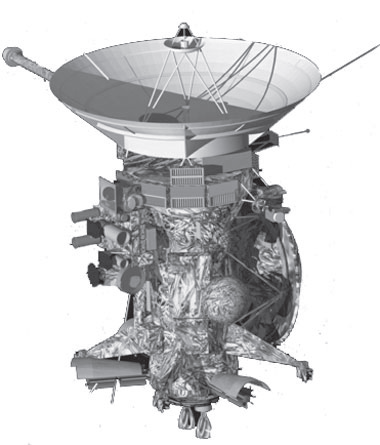
\includegraphics[width=4cm]{fig_00} \\
\textit{Représentation ciculaire du métro parisien}
}%figues de la page de garde


\input{\repRel/Style/pagegarde_cours_minitoc}
\setlength{\columnseprule}{.1pt}

\vspace{2cm}
\pagestyle{fancy}
\thispagestyle{plain}

%Thème : Tris.
% 
%Commentaires :
%\begin{itemize}
%\item algorithmique quadratique : tri par insertion, par sélection;
%\item tri par partition-fusion;
%\item tri par comptage.
%\end{itemize}
%\textit{On fait observer différentes caractéristiques (par exemple2 stable ou non, en place ou non, comparatif ou non ...).}
%


\section{Introduction}
Historiquement, le problème des sept ponts de Königsberg (Kaliningrad) était de déterminer s'il existe une promenade qui partait de n'importe quel quartier et qui y revenait, tout en passant une et une seule fois par chacun des ponts.
Euler mis en forme le problème et le résolut... en montrant que dans ce cas, il n'existait pas de solution.
\begin{center}
\begin{tabular}{cccc}
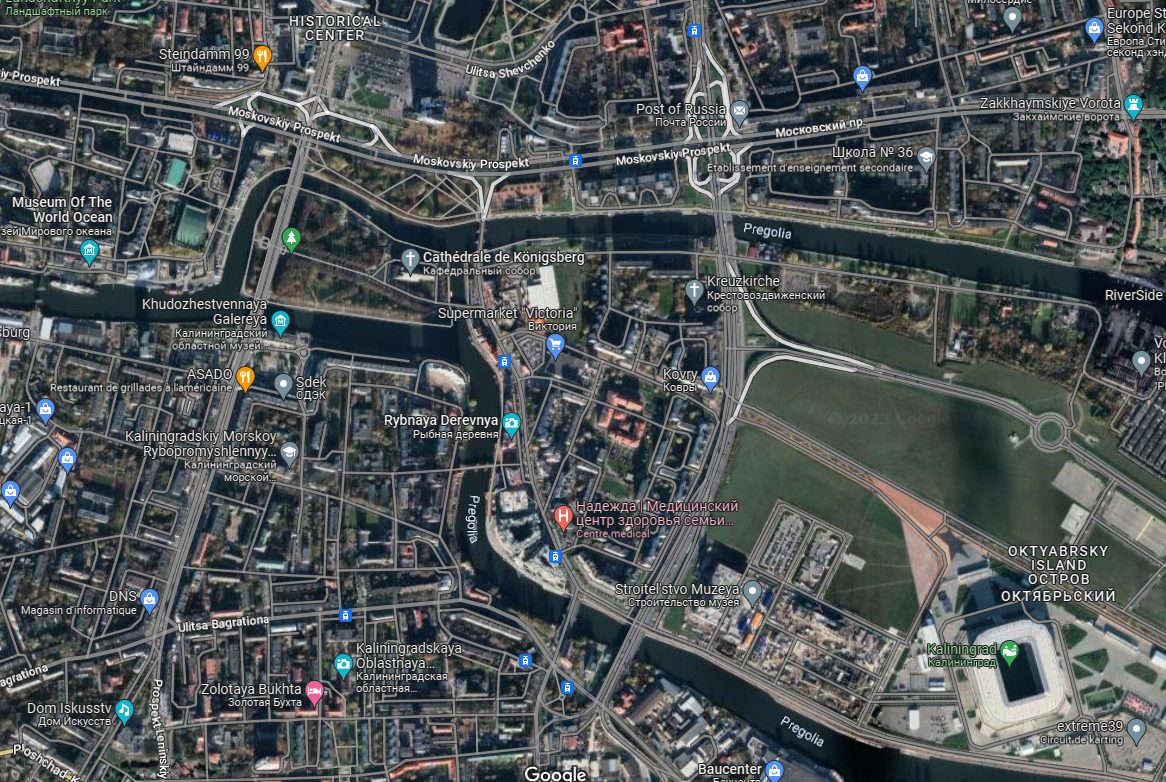
\includegraphics[width=0.2\linewidth]{konigsberg_01} &
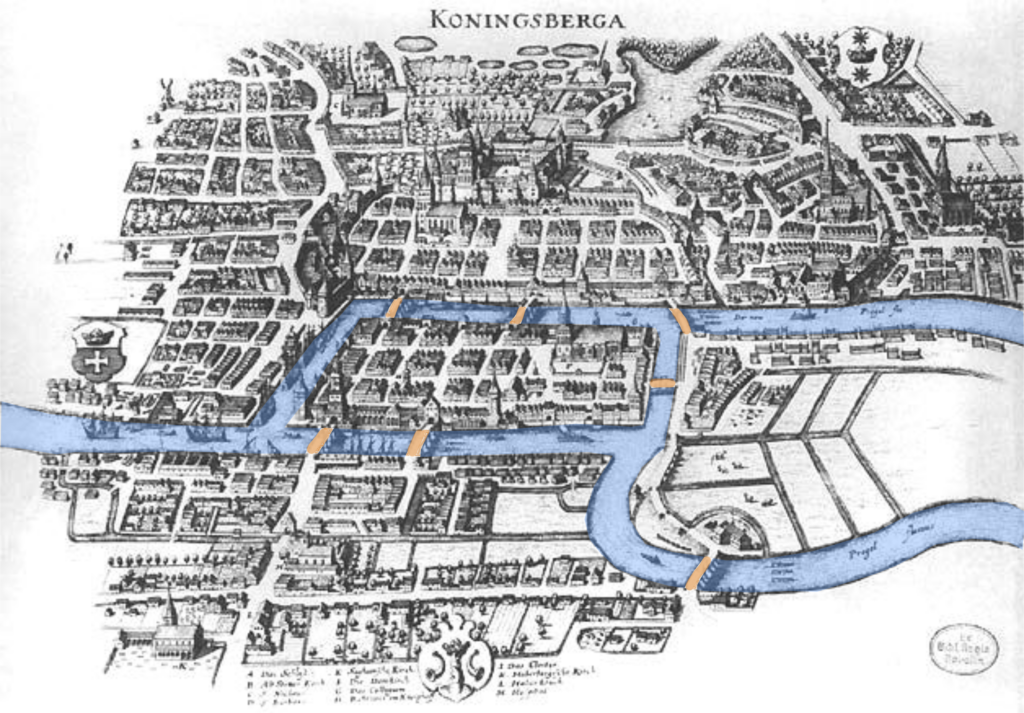
\includegraphics[width=0.2\linewidth]{konigsberg_02} &
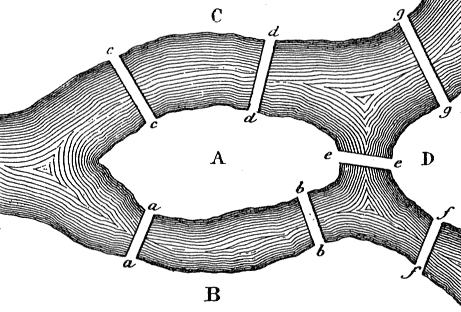
\includegraphics[width=0.2\linewidth]{konigsberg_03} &
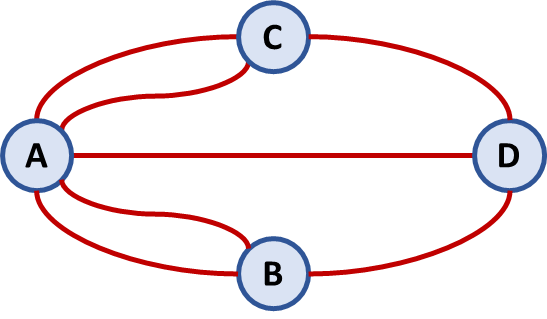
\includegraphics[width=0.2\linewidth]{konigsberg_04} \\
\end{tabular}
\end{center}

Les applications des graphes sont assez nombreuses :
\begin{itemize}
 \item recherche d'itinéraire pour aller d'un point à un autre;
 \item rourage des paquets sur Internet;
 \item analyse des réseaux sociaux...
 \end{itemize}
 

\section{Vocabulaire des graphes}

\begin{defi}{Graphe}%\cite{ref_01}
Un graphe est un ensemble de \textbf{sommets} et  \textbf{relations} entre ces sommets.

Lorsque deux sommets sont en relation, on dit qu'il existe une \textbf{arête} entre ces sommets.
\end{defi}

\begin{defi}{Graphe non orienté -- Arêtes}
Un graphe non orienté $G$ est un couple $G=(S,A)$, où $S$ est un ensemble fini de sommets (appelés aussi n\oe uds)  et où $A$ est un ensemble fini de paires ordonnées de sommets, appelées arêtes.

On note $x - y$ l'arête $\{x,y\}$. $x$ et $y$ sont les deux extrémités de l'arête.
\end{defi}

\begin{defi}{Graphe orienté -- Arcs}\cite{ref_01}
Un graphe orienté $G$ est un couple $G=(S,A)$, où $S$ est un ensemble fini de sommets et où $A$ est un ensemble fini de paires ordonnées de sommets, appelées arcs.

On note $x\to y$ l'arc $(x,y)$. $x$ est l'extrémité initiale de l'arc, $y$ est son extrémité terminale. On dit que $y$ est successeur de $x$ et que $x$ est prédécesseur de $y$. 
\end{defi}

\begin{exemple}~\\

\begin{multicols}{2}
\begin{figure}[H]
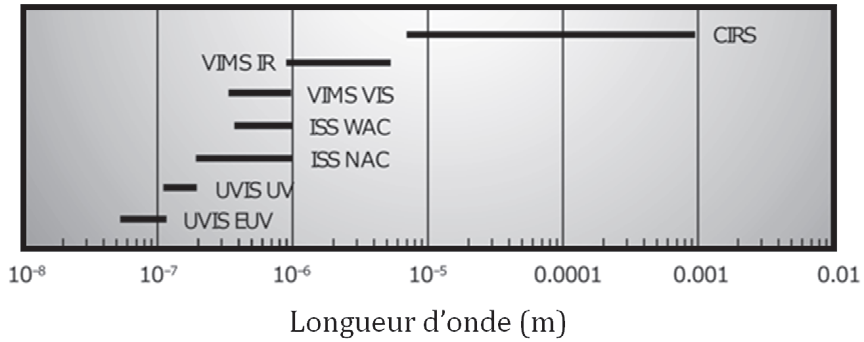
\includegraphics[width=.8\linewidth]{fig_02}
\captionsetup{justification=centering}
\caption{Graphe non orienté \label{fig_02}}
\end{figure}


\begin{figure}[H]
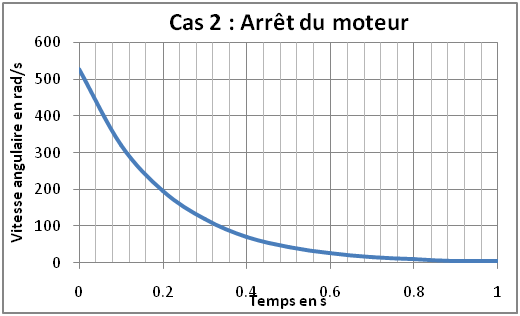
\includegraphics[width=.8\linewidth]{fig_03}
\captionsetup{justification=centering}
\caption{Graphe orienté}
\end{figure}
\end{multicols}

\end{exemple}

\begin{rem}
On peut noter le graphe non orienté $G=\left(\llbracket 1,6\rrbracket,E\right)$ où $E=\left(
\left\{1,2\right\},\left\{2,3\right\},\left\{3,4\right\},\left\{1,4\right\},\left\{1,3\right\},\left\{1,5\right\},\left\{1,6\right\}\right)$ désigne les arêtes. 

On peut noter le graphe orienté $G=\left(\llbracket 1,6\rrbracket,E\right)$ où $E=\left(
\left(1,2\right),\left(2,3\right),\left(3,4\right),\left(1,4\right),\left(1,3\right),\left(1,5\right),\left(1,6\right)\right)$ désigne les arcs. 
\end{rem}

\begin{defi}{Adjacence}
Deux arcs (resp. arêtes) d'un graphe orienté (resp. non orienté) sont dits adjacents s'ils ont au moins une extrémité commune. 

Deux sommets d'un graphe non orienté sont dits adjacents s'il existe une arête les joignant. 

Dans un graphe orienté, le sommet $y$ est dit adjacent au sommet $x$ s'il existe un arc $x\to y$.
\end{defi}


\begin{defi}{Graphes pondérés}
Étiqueter les arêtes d’un graphe $(S, A)$ (orienté ou non), c’est se donner une fonction
$f : A \to V$ (où $V$ est un ensemble de valeurs). On dit qu’un graphe est pondéré si ses arêtes sont étiquetées par des nombres. On parlera alors du poids d’une arête.
\end{defi}
%
%\begin{defi}{Sommet (ou n\oe{}uds)}
%\end{defi}
%
%\begin{defi}{Arc, arête}
%\end{defi}

\section{Chemins}

\begin{defi}{Chemin dans un graphe} \\

\noindent\begin{minipage}{.7\linewidth}
On appelle chemin dans un graphe une suite finie $\{S_0, \ldots , S_{n-1}\}$ de $n$ sommets tels que pour tout
$i \in \llbracket 0, n-1\llbracket$, une arête relie $S_i$ à $S_{i+1}$. On dit que ce chemin relie le sommet de départ $S_0$ au sommet de fin $S_{n-1}$. 

Dans le cas d'un graphe non orienté, les arêtes sont notées $\{S_i, S_{i+1}\}$ pour $i \in \llbracket 0, n-1\llbracket$.

Dans le cas d'un graphe orienté, les arcs sont notées $(S_i, S_{i+1})$ pour $i \in \llbracket 0, n-1\llbracket$.
\end{minipage}\hfill
\begin{minipage}{.25\linewidth}
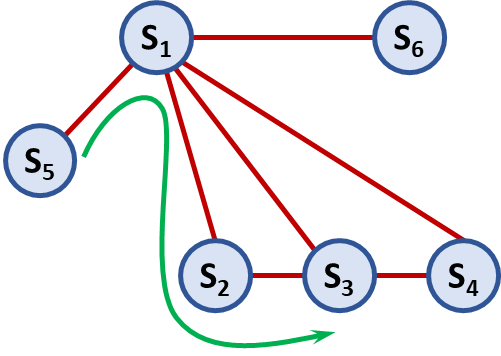
\includegraphics[width=\linewidth]{chemin}
\end{minipage}
\end{defi}

\begin{defi}{Chemin fermé} \\

\noindent\begin{minipage}{.7\linewidth}
Chemin dont le sommet de départ et le sommet d'arrivée sont identiques.
\end{minipage}\hfill
\begin{minipage}{.25\linewidth}
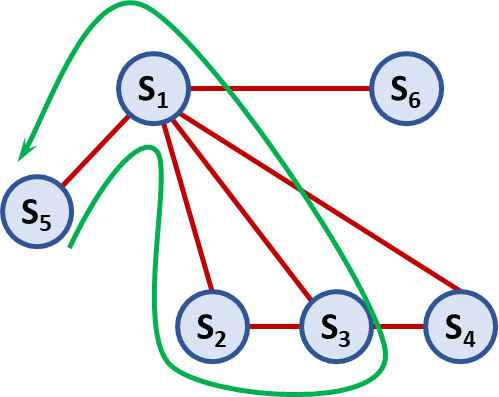
\includegraphics[width=\linewidth]{cycle_simple}
\end{minipage}

\end{defi}

\begin{defi}{Chemin élémentaire}

\noindent\begin{minipage}{.7\linewidth}
Chemin n'empruntant que des arêtes distinctes.
\end{minipage} \hfill
\begin{minipage}{.25\linewidth}
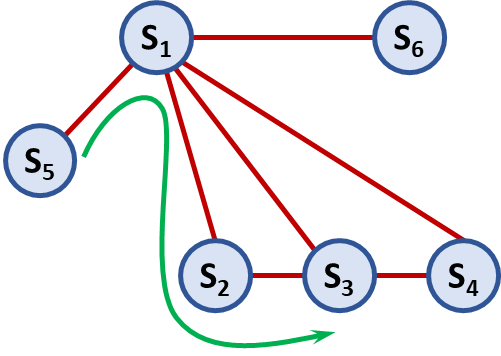
\includegraphics[width=\linewidth]{chemin}
\end{minipage}
\end{defi}

\begin{defi}{Chemin simple}
Chemin tel que les $n - 2$ sommets intermédiaires si, pour $i \in \llbracket 1, n-1\llbracket$ soient
deux à deux distincts et tous distincts du sommet de départ $S_0$ et du sommet d’arrivée $S_{n-1}$ et tels
que ce chemin n’est pas de la forme $a, b, a$ dans le cas non-orienté.
\end{defi}

\begin{defi}{Circuit}
Chemin fermé de longueur non nulle.
\end{defi}


\begin{defi}{Cycle}
Circuit élémentaire (chemin fermé de longueur non nulle dont toutes les arêtes sont distinctes).
\end{defi}

\begin{defi}{Cycle simple} 
Chemin fermé et simple de longueur non nulle.
\end{defi}

\begin{defi}{Chemin et cycle eulérien}

\noindent\begin{minipage}{.55\linewidth}
Chemin (resp. cycle) contenant une et une seule fois toutes les arêtes du graphe.
%Graphe eulérien : contenant un circuit eulérien.
%Graphe acyclique : ne contenant aucun cycle.
\end{minipage} \hfill
\begin{minipage}{.2\linewidth}
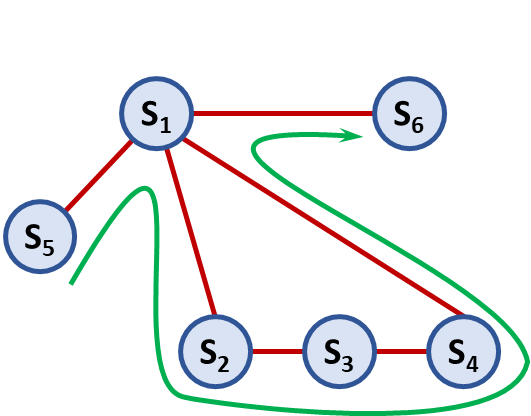
\includegraphics[width=\linewidth]{chemin_eulerien}
\end{minipage}
 \hfill
\begin{minipage}{.2\linewidth}
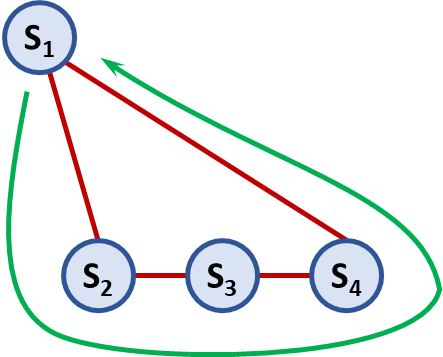
\includegraphics[width=\linewidth]{cycle_eulerien}
\end{minipage}
\end{defi}

\begin{rem}
Pour certains auteurs, un chemin élémentaire est ce que nous avons appelé un chemin simple et réciproquement. Pour d’autres, un cycle est ce que nous avons appelé un cycle simple.
\end{rem}

%
%\begin{exemple} ~\\
%\begin{multicols}{2}
%\begin{figure}[H]
%\centering
%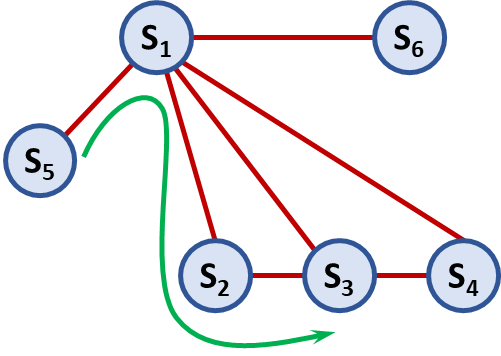
\includegraphics[height = 4cm]{chemin}
%\captionsetup{justification=centering}
%\caption{Chemin}
%\end{figure}
%
%\begin{figure}[H]
%\centering
%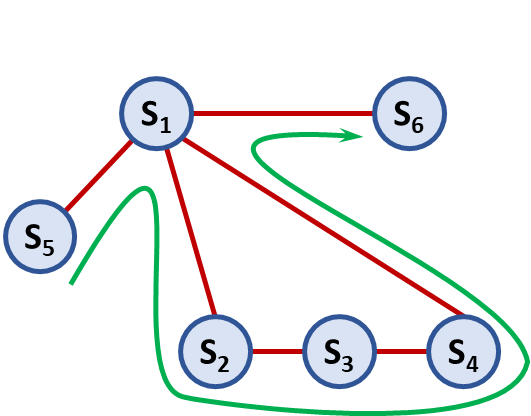
\includegraphics[height = 4cm]{chemin_eulerien}
%\captionsetup{justification=centering}
%\caption{Chemin eulérien}
%\end{figure}
%
%\begin{figure}[H]
%\centering
%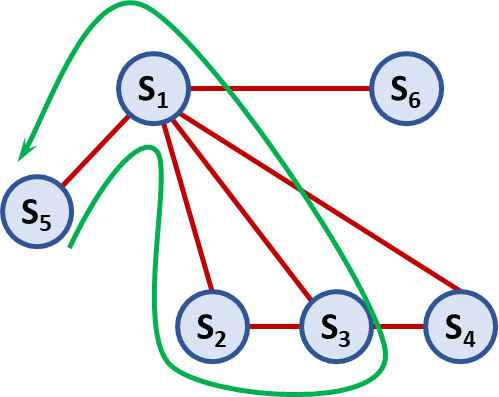
\includegraphics[height = 4cm]{cycle_simple}
%\captionsetup{justification=centering}
%\caption{Cycle simple}
%\end{figure}
%
%\begin{figure}[H]
%\centering
%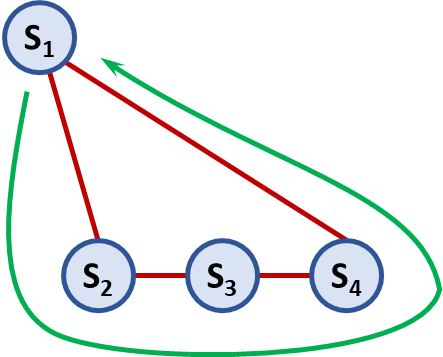
\includegraphics[height = 4cm]{cycle_eulerien}
%\captionsetup{justification=centering}
%\caption{Cycle eulérien}
%\end{figure}
%\end{multicols}
%\end{exemple}


%\begin{defi}{}
%\end{defi}
%
%\begin{defi}{}
%\end{defi}



\begin{defi}{Connexité dans les graphes non orientés}
Un graphe $G=(S,A)$ est dit connexe si, pour deux sommets quelconques $S_i$ et $S_j$ de $S$, il existe un chemin de $S_i$ à $S_j$.
\end{defi}

\begin{exemple}
\begin{figure}[H]
\centering
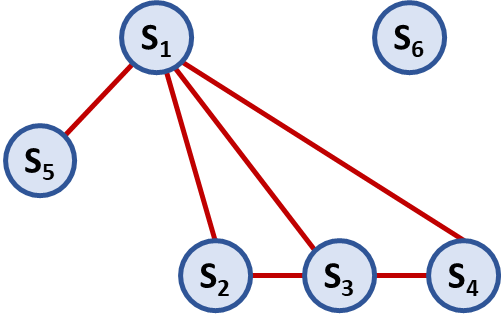
\includegraphics[height = 4cm]{connexite}
\captionsetup{justification=centering}
\caption{Graphe ayant 2 composantes connexes}
\end{figure}
\end{exemple}

\subsection{Notations}
\begin{defi}{Degré d'un sommet}
On appelle degré d'un sommet $s$ et on note $d\left(s\right)$ le nombres d'arcs (ou d'arêtes) dont $s$ est une extrémité.
\end{defi}

\begin{defi}{Degré entrant et sortant}
On note $s$ le sommet d'un graphe orienté. On note : 
\begin{itemize}
\item $d_{+}\left(s\right)$ le demi-degré extérieur de $s$, c'est-à-dire le nombre d'arcs ayant leur extrémité initiale en $s$ (ces arcs sont dits incidents à $s$ vers l'extérieur);
\item $d_{-}\left(s\right)$ le demi-degré intérieur de $s$, c'est-à-dire le nombre d'arcs ayant leur extrémité finale en $s$ (ces arcs sont dits incidents à $s$ vers l'intérieur).
\end{itemize}

Dans ce cas, on a  $d\degres\left(s\right)=d_{-}\left(s\right)+d_{+}\left(s\right)$.
\end{defi}


\begin{exemple}~\\

\begin{multicols}{2}
\begin{figure}[H]
\centering
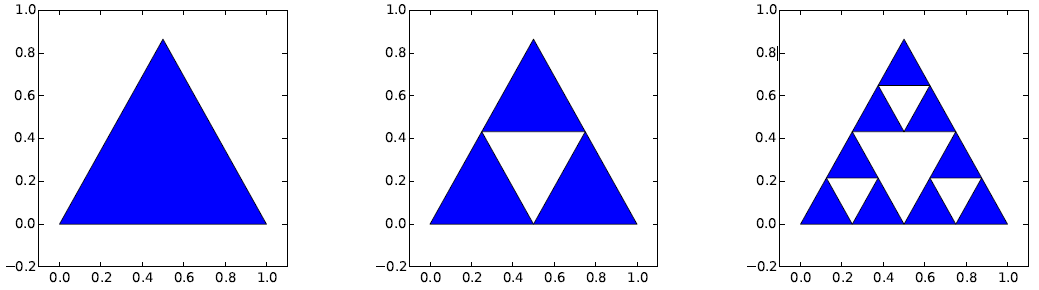
\includegraphics[width=.8\linewidth]{fig_04}
\captionsetup{justification=centering}
\caption{Graphe orienté \label{fig_04}}
\end{figure}

\begin{itemize}
\item $d_{-}\left(S_1\right)=3$.
\item $d_{+}\left(S_1\right)=4$.
\item $d\degres\left(S_1\right)=7$.
\end{itemize}
\end{multicols}

\end{exemple}

\section{Implémentation des graphes}

\subsection{Liste d'adjacence}
\begin{defi}{Liste d'adjacence}
Soit un graphe de $n$ sommets d'indices $i \in \llbracket 0, n-1\rrbracket$. Pour implémenter le graphe, on utilise une liste \texttt{G} de taille $n$ pour laquelle, \texttt{G[i]} est la liste des voisins de \texttt{i}.
\end{defi}
\begin{rem}
Cette implémentation est plutôt réservée au graphes << creux >>, c'est-à-dire ayant peu d'arêtes.
\end{rem}

\begin{exemple} ~\\
\begin{minipage}[b]{.47\linewidth}
\begin{center}
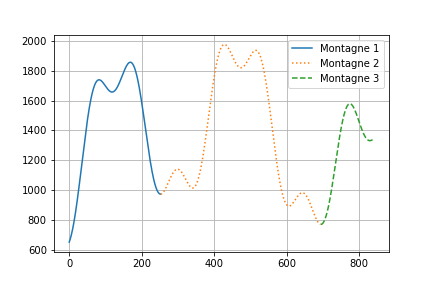
\includegraphics[width=.7\linewidth]{fig_05}
\end{center}
Dans ce cas $S_0$ est voisin de $S_1$, $S_5$ et $S_6$; donc \texttt{G[0]=[1,5,6]}. 
$S_3$ est voisin de $S_2$ et $S_4$; donc \texttt{G[3]=[2,4]}.
\begin{lstlisting}
G = [[1,5,6],[0,2,6],[1,3],[2,4],[3,5],
      [4,0],[1,0]]
\end{lstlisting}
\end{minipage}\hfill
\begin{minipage}[b]{.47\linewidth}
\begin{center}
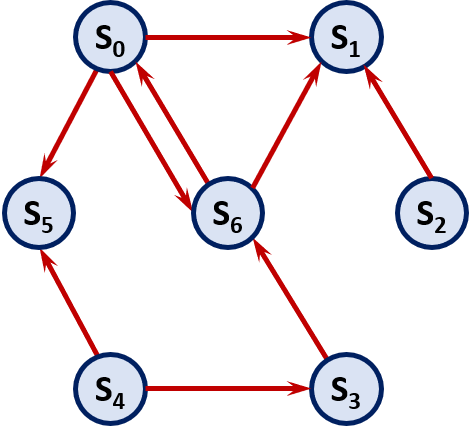
\includegraphics[width=.7\linewidth]{fig_06}
\end{center}
Dans ca cas, le graphe est orienté. La liste d'adjacence contient la liste des successeurs. Ainsi, les successeurs de $S_0$ sont $S_1$, $S_5$ et $S_6$; donc \texttt{G[0]=[1,5,6]}. $S_1$ n'a pas de successeur donc \texttt{G[1]=[]}.
\begin{lstlisting}
G = [[1,5,6],[],[1],[6],[3,5],[],[0,1]]
\end{lstlisting}
\end{minipage}
\end{exemple}


\subsection{Dictionnaire d'adjacence}

Dans la même idée, il est aussi possible d'utiliser des dictionnaires d'adjacence dans lequel les clés sont les sommets (qui peuvent être des entiers ou des chaînes de caractères), et les valeurs sont des listes de voisins ou de successeurs (qui peuvent donc être des listes d'entiers ou de chaînes de caractères).

\begin{lstlisting}
# Graphe non orienté 
G = {"S0":["S1","S5","S6"],"S1":["S0","S2","S6"],"S2":["S1","S3"],"S3":["S2","S4"],"S4":["S3","S5"],"S5":["S4","S0"],"S6":["S1","S0"]}
# Graphe orienté 
G = {"S0":["S1","S5","S6"],"S1":[],"S2":["S1"],"S3":["S6"],"S4":["S3","S5"],"S5":[],"S6":["S1","S0"]}
\end{lstlisting}

\subsection{Matrice d'adjacence}
\begin{defi}{Matrice d'adjacence}
Soit un graphe de $n$ sommets d'indices $i \in \llbracket 0, n-1\rrbracket$ et $E$ l'ensemble des arêtes 
(on notera $G=\left( \llbracket 0, n-1\rrbracket,E\right)$. Pour implémenter le graphe, on utilise la matrice d'adjacence carrée de taille $n$, $\mathcal{M}_n$ \texttt{G} de taille $n$ pour laquelle,
$m_{i,j}=\left\{
\begin{array}{l}
\texttt{True } \text{ si } \{i,j\}\in E\\
\texttt{False } \text{ sinon } 
\end{array}
\right.$ avec $i,j\in \llbracket 0, n-1\rrbracket$. 


\end{defi}
\begin{rem}
Cette implémentation est plutôt réservée au graphes << denses >> ayant << beaucoup >> d'arêtes.
\end{rem}


\begin{exemple} ~\\
\begin{minipage}[b]{.47\linewidth}
\begin{center}
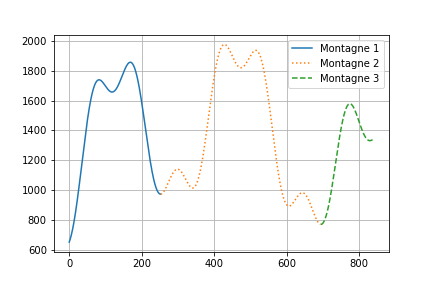
\includegraphics[width=.7\linewidth]{fig_05}
\end{center}

On a dans ce cas 

\footnotesize{$
M = $

$
\begin{pmatrix}
\texttt{False} & \texttt{True} & \texttt{False} & \texttt{False} & \texttt{False} & \texttt{True} & \texttt{True} \\
\texttt{True} & \texttt{False} & \texttt{True} & \texttt{False} & \texttt{False} & \texttt{False} & \texttt{True} \\ 
\texttt{False} & \texttt{True} & \texttt{False} & \texttt{True} & \texttt{False} & \texttt{False} & \texttt{False} \\
\texttt{False} & \texttt{False} & \texttt{True} & \texttt{False} & \texttt{True} & \texttt{False} & \texttt{False} \\
\texttt{False} & \texttt{False} & \texttt{False} & \texttt{True} & \texttt{False} & \texttt{True} & \texttt{False} \\
\texttt{True} & \texttt{False} & \texttt{False} & \texttt{False} & \texttt{True} & \texttt{False} & \texttt{False} \\
\texttt{True} & \texttt{True} & \texttt{False} & \texttt{False} & \texttt{False} & \texttt{False} & \texttt{False} \\
\end{pmatrix}$}

ou 

\footnotesize{$
M = 
\begin{pmatrix}
\texttt{0} & \texttt{1} & \texttt{0} & \texttt{0} & \texttt{0} & \texttt{1} & \texttt{1} \\
\texttt{1} & \texttt{0} & \texttt{1} & \texttt{0} & \texttt{0} & \texttt{0} & \texttt{1} \\ 
\texttt{0} & \texttt{1} & \texttt{0} & \texttt{1} & \texttt{0} & \texttt{0} & \texttt{0} \\
\texttt{0} & \texttt{0} & \texttt{1} & \texttt{0} & \texttt{1} & \texttt{0} & \texttt{0} \\
\texttt{0} & \texttt{0} & \texttt{0} & \texttt{1} & \texttt{0} & \texttt{1} & \texttt{0} \\
\texttt{1} & \texttt{0} & \texttt{0} & \texttt{0} & \texttt{1} & \texttt{0} & \texttt{0} \\
\texttt{1} & \texttt{1} & \texttt{0} & \texttt{0} & \texttt{0} & \texttt{0} & \texttt{0} \\
\end{pmatrix}$}


\end{minipage}\hfill
\begin{minipage}[b]{.47\linewidth}
\begin{center}
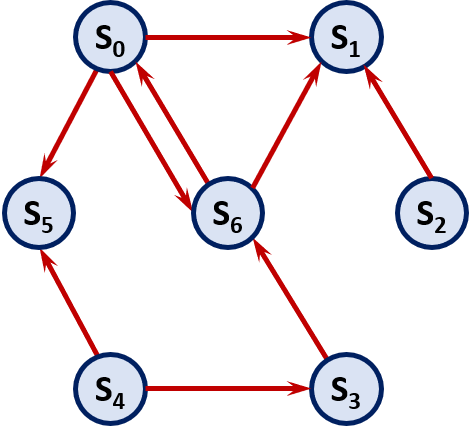
\includegraphics[width=.7\linewidth]{fig_06}
\end{center}
Dans ce cas, le graphe est orienté.
On a dans ce cas 

\footnotesize{$
M = $

$
\begin{pmatrix}
\texttt{False} & \texttt{True} & \texttt{False} & \texttt{False} & \texttt{False} & \texttt{True} & \texttt{True} \\
\texttt{False} & \texttt{False} & \texttt{False} & \texttt{False} & \texttt{False} & \texttt{False} & \texttt{False} \\ 
\texttt{False} & \texttt{True} & \texttt{False} & \texttt{False} & \texttt{False} & \texttt{False} & \texttt{False} \\
\texttt{False} & \texttt{False} & \texttt{False} & \texttt{False} & \texttt{False} & \texttt{False} & \texttt{True} \\
\texttt{False} & \texttt{False} & \texttt{False} & \texttt{True} & \texttt{False} & \texttt{True} & \texttt{False} \\
\texttt{False} & \texttt{False} & \texttt{False} & \texttt{False} & \texttt{False} & \texttt{False} & \texttt{False} \\
\texttt{True} & \texttt{True} & \texttt{False} & \texttt{False} & \texttt{False} & \texttt{False} & \texttt{False} \\
\end{pmatrix}$}

ou 
\footnotesize{$
M =
\begin{pmatrix}
\texttt{0} & \texttt{1} & \texttt{0} & \texttt{0} & \texttt{0} & \texttt{1} & \texttt{1} \\
\texttt{0} & \texttt{0} & \texttt{0} & \texttt{0} & \texttt{0} & \texttt{0} & \texttt{0} \\ 
\texttt{0} & \texttt{1} & \texttt{0} & \texttt{0} & \texttt{0} & \texttt{0} & \texttt{0} \\
\texttt{0} & \texttt{0} & \texttt{0} & \texttt{0} & \texttt{0} & \texttt{0} & \texttt{1} \\
\texttt{0} & \texttt{0} & \texttt{0} & \texttt{1} & \texttt{0} & \texttt{1} & \texttt{0} \\
\texttt{0} & \texttt{0} & \texttt{0} & \texttt{0} & \texttt{0} & \texttt{0} & \texttt{0} \\
\texttt{1} & \texttt{1} & \texttt{0} & \texttt{0} & \texttt{0} & \texttt{0} & \texttt{0} \\
\end{pmatrix}$}

\end{minipage}
\end{exemple}


\begin{rem}
\begin{itemize}
\item Dans le cas d'un graphe non orienté, la matrice est symétrique. 
\item Si on avait un bouclage sur un sommet, il y aurait des valeurs non nulles sur la diagonale. 
\end{itemize}
\end{rem}

\subsection{Graphes pondérés}
Une matrice de pondatération est une matrice d'adjacence adaptée : 
\begin{itemize}
\item $M[i][j] = w_{ij}$ s’il y a un arc de poids $w_{ij}$ d’extrémité initiale $s_i$ et d’extrémité terminale $s_j$ ;
\item $M[i][j] = 0$ (ou $M[i][j] = \infty$) s’il n’existe pas un arc d’extrémité initiale $s_i$ et d’extrémité
terminale $s_j$ .
\end{itemize}
%\section{Parcours d'un graphe}
%
%Une fois un graphe implémenté, se pose la question du parcours de ce graphe. Par exemple, pour aller de Monplaisir à La Part-Dieu en transport en commun, quel sera le parcours le plus rapide ? le plus court ? le moins énergivore ?
%
%Il faudrait alors tester tous les chemins possibles entre deux points, puis les comparer selon des critères prédéfinis. 
%
%Afin de créer, gérer, stocker ces parcours, on pourra implémenter les chemins parcourus sous forme de \textbf{file} ou \textbf{pile}.
%
%\subsection{Piles et files}
%
%\subsubsection{Pile}
%\begin{defi}{Pile}
%Une pile est une structure de données dans laquelle le dernier élément stocké est le premier à en sortir. On parle de principe \textit{LIFO} pour \textit{Last In First Out}. Le dernier élément stocké est appelé \textbf{sommet}.
%\end{defi}
%
%Pour gérer une pile, indépendamment de la façon dont elle est implémentée, on suppose exister les opérations élémentaires suivantes : 
%\begin{itemize}
%\item création d'une pile vide;
%\item test si une pile est vide;
%\item rajout d'un élément au sommet de la pile;
%\item accès au sommet d'une pile non vide;
%\item suppression (et renvoi) du sommet d'une pile non vide.
%\end{itemize}
%
%Théoriquement, chacune de ces opérations doit se faire à \textbf{temps constant}.
%
%Une des possiblités pour implémenter les piles est d'utiliser le module \texttt{deque}. Chacun des éléments de la pile peut être un objet de type différent.
%
%\begin{lstlisting} 
%from collections import deque
%
%# Création d'une pile vide
%pile = deque() 
%
%# Test si une pile est vide
%len(pile) == 0
%
%# Ajout de l'élément Truc au sommet de la pile
%pile.append("Truc")
%
%# Suppression (et renvoi) du sommet d'une pile non vide
%sommet = pile.pop()
%\end{lstlisting}
%
%
%
%\subsubsection{File}
%\begin{defi}{File}
%Une file est une structure de données dans laquelle le premier élément stocké est le premier à en sortir. On parle de principe \textit{FIFO} pour \textit{First In First Out}. 
%\end{defi}
%
%Pour gérer une file, indépendamment de la façon dont elle est implémentée, on suppose exister les opérations élémentaires suivantes : 
%\begin{itemize}
%\item création d'une file vide;
%\item test si une file est vide;
%\item rajout d'un élément dans la file;
%\item suppression (et renvoi) du premier élément innséré dans la file.
%\end{itemize}
%
%Théoriquement, chacune de ces opérations doit se faire à \textbf{temps constant}.
%
%Une des possiblités pour implémenter les piles est d'utiliser le module \texttt{deque}. Chacun des éléments de la file peut être un objet de type différent. Dans cette vision des files, les éléments sont ajoutés << à droite >> et sortent de la file << par la gauche >>.
%
%\begin{lstlisting} 
%from collections import deque
%
%# Création d'une file vide
%file = deque() 
%
%# Teste si une pile est vide
%len(file) == 0
%
%# Ajoute l'élément Truc dans la file 
%file.append("Truc")
%
%# Suppression (et renvoi) du premier élément inséré dans la file
%sommet = pile.popleft()
%
%\end{lstlisting}
%
%
%\subsection{Parcours générique d'un graphe}
%
%\begin{defi}{Parcours générique}
%Soit in graphe $G=(S,A)$. On parle de parcours générique d'un graphe lorsqu'on souhaite savoir, à partir du sommet $S_i$, quels sont les sommets accessibles. 
%\end{defi}
%
%\subsection{Parcours en largeur}
%
%\subsection{Parcours en profondeur}
%
%\subsection{Détection de la présence des cycles}
%
%\subsection{Connexité d'un graphe non orienté}
%
%\section{Pondération d'un graphe}
%
%
%
%\section{Recheche du plus court chemin}
%\subsection{Algorithme de Dijkstra}
%
%\subsection{Algorithme A$\star$}
%
%\begin{defi}{}
%\end{defi}
%
%\begin{defi}{}
%\end{defi}
%
%\begin{defi}{}
%\end{defi}
%
%\begin{defi}{}
%\end{defi}
%
%\begin{defi}{}
%\end{defi}


\subsection{Taille d'un graphe}

\begin{defi}{Taille d'un graphe}
Soit un graphe $G=\left(V,E\right)$ composé de sommets $V$ et d'arêtes $E$. On appelle taille du graphe la quantité $|V|+|E|$.
\end{defi}

\begin{rem}
On retrouve dans des ouvrages la notation $|V|$ ou $|E|$ correspondant respectivement au nombre de sommets et d'arêtes. 
Ainsi, si un algorithme est linéaire en la taille du graphe, on pourra utilisé la notation $\mathcal{O}\left(|V|+|E|\right)$.
\end{rem}

\subsection{Formule des degrés}
\begin{defi}{Formule des degrés}
Soit un graphe $G=\left(V,E\right)$, alors : $\displaystyle{\Sigma_{v \in V}} \text{deg}(v) = 2|E|$.
\end{defi}

\subsection{Graphe complet}

\begin{defi}{Graphe complet}
Un graphe complet est un graphe possédant toutes les arêtes possibles. 
\end{defi}

\begin{rem}
\begin{itemize}
\item Le nombre maximal d'arêtes d'un graphe à $n$ sommets est donné par : $\begin{pmatrix} n \\ 2\end{pmatrix}$.
\item Pour chaque sommet $v$ on a $d\degres (v) = n-1$.
\item Le nombre d'arêtes est en $\mathcal{O}\left(|V|^2\right)$.
\end{itemize}
\end{rem}

\subsection{Matrices d'adjacences}

\begin{minipage}[t]{.47\linewidth}
\begin{center}
\textbf{Avantages}
\end{center}
\begin{itemize}
\item Le test d’adjacence de deux sommets se fait en temps constant.
\item Dans le cas d’un graphe orienté, obtenir les prédécesseurs n’est pas plus compliqué (ni plus coûteux)
que d’obtenir les successeurs.
\item Rajouter ou supprimer une arête (ou un arc) peut se faire en temps constant.
%\item Il est possible de n’utiliser qu’un bit par coefficient de la matrice : dans le cas d’un graphe dense,
%une telle représentation est donc très compacte.
\end{itemize}
\end{minipage}
\hfill
\begin{minipage}[t]{.47\linewidth}
\begin{center}
\textbf{Inconvénients}
\begin{itemize}
\item Ajouter ou supprimer un sommet nécessite un temps proportionnel à $n^2$.
\item Pour récupérer les voisins/successeurs d’un nœud, il faut parcourir toute la ligne de la matrice :
l’opération se fait donc en$\mathcal{O}(n)$\footnote{$\Theta(n)$}, ce qui est regrettable si le degré sortant du noeud est petit devant $n$.
\item On consomme une mémoire proportionnelle à $|V|^2$, même quand la taille du graphe est de l’ordre de $n$ (graphe creux).
\end{itemize}
\end{center}
\end{minipage}

\subsection{Listes d'adjacences}

\begin{minipage}[t]{.47\linewidth}
\begin{center}
\textbf{Avantages}
\end{center}
\begin{itemize}
\item La mémoire utilisée est de l’ordre de $|E| + |V|$, ce qui est nettement mieux que $|V|^2$ si le graphe est
creux.
\item On a directement accès à la liste des voisins d’un noeud : la parcourir prend un temps proportionnel
au degré sortant du noeud.% (et pas à $|V|$).
\item Ajouter un noeud peut normalement se faire en temps $|V|$ (si l’ajout n’impose pas de renuméroter
les noeuds déjà présents).
\end{itemize}
\end{minipage}
\hfill
\begin{minipage}[t]{.47\linewidth}
\begin{center}
\textbf{Inconvénients}
\begin{itemize}
%\item  Si l’on a besoin d’un accès en temps raisonnable aux prédécesseurs d’un noeud (dans le cas orienté),
%il faut stocker séparément le tableau de listes correspondant.
\item Le test d’adjacence ne se fait plus en temps constant (mais en temps proportionnel au degré du
nœud).
\item Si le graphe est dense, on consommera plus de mémoire (d’un facteur constant) qu’avec une matrice
d’adjacence.
\item Ajouter ou supprimer une arête n’est pas aussi évident que dans une matrice d’adjacence : suivant
l’opération précise que l’on souhaite faire, la complexité peut être unitaire ou proportionnelle aux
degrés des nœuds impactés.
\item  Supprimer un noeud n’est pas pratique : le plus simple est de reconstruire entièrement le graphe (en
un temps $\mathcal{O}\left(|E| + |V|\right)$).
\end{itemize}
\end{center}
\end{minipage}

\section{Applications}

\subsection{Exemple d'implémentation d'après un sujet de l'XENS 2015}
On souhaite stocker en mémoire une liste non-ordonnée d'au plus n entiers sans redondance (i.e. ou aucun entier n'apparaît
plusieurs fois). Nous utilisons un tableau 
liste de longueur $n+1$ tel que :
\begin{itemize}
\item liste\verb![!0\verb!]! contient le nombre d'éléments dans le tableau ;
\item liste\verb![!i\verb!]! contient le i\ieme élément de la liste non-ordonnée avec $1\leqslant i \leqslant $\texttt{liste[0]}.
\end{itemize}
Nous disposons d'une fonction \texttt{creerListeVide(n:int)->list} qui permet de créer une liste pouvant contenir $n$ éléments.

\begin{lstlisting}
>>> creerListeVide(3)
        [0,None,None,None]
\end{lstlisting}

Nous disposons d'une fonction \texttt{estDansListe(liste:list,x)->bool} qui renvoie \texttt{True} si l'élément $x$ est dans la liste et \texttt{False} sinon.

La complexité de cette fonction est linéaire en fonction du nombre d'élément maximum que peut contenir la liste. 
Nous disposons aussi d'une fonction \texttt{ajouteDansListe(liste:list,x)} qui modifie la liste pour ajouter l'élément $x$ s'il n'est pas présent et ne fait rien sinon. La complexité est aussi linéaire du nombre d'élément maximum que peut contenir la liste.

Un plan $P$ est défini par un ensemble de $n$ villes numérotées de $1$ à $n$ et un ensemble de $m$ routes (toutes à double sens)
reliant chacune deux villes. On dira que deux villes $x, y \in  n$ sont voisines lorsqu'elles sont reliées par une route, ce que l'on notera $(x, y)$. On appellera chemin de longueur $k-1$ toute suite de villes $\verb![!v_1, v_2 ... , v_k\verb!]!$. Un plan $P$ est alors un graphe dont les sommets sont les villes et les routes les arêtes.

\textbf{Structure de données. } 

Nous représentons tout plan $P$ à $n$ villes par un tableau plan de $(n+1)$ tableaux où :
\begin{itemize}
\item plan\verb![!0\verb!]! contient un tableau de deux éléments où :
\begin{itemize}
\item plan\verb![!0\verb!]!\verb![!0\verb!]! a pour valeur le nombres $n$ de villes;
\item plan\verb![!0\verb!]!\verb![!1\verb!]! a pour valeur le nombres $m$ de routes.
\end{itemize}
\end{itemize}


\begin{itemize}
\item Pour toute ville $v \in n$, plan\verb![!v\verb!]! contient un tableau à $n$ éléments représentant 
la liste à au plus $(n-1)$ éléments des villes voisines de $v$ dans $P$ dans un ordre arbitraire en utilisant
la structure de liste sans redondance décrite plus haut. Ainsi :
\begin{itemize}
\item plan\verb![!v\verb!]!\verb![!0\verb!]! a pour valeur le nombre de villes voisines de $v$ ;
\item plan\verb![!v\verb!]!\verb![!1\verb!]! , ... ,n\verb![!v\verb!]!\verb![!n\verb![!v\verb!]!\verb![!0\verb!]!\verb!]! sont les indices des villes voisines de $v$.
\end{itemize}
\end{itemize}

\begin{minipage}[c]{.45\linewidth}
\begin{center}
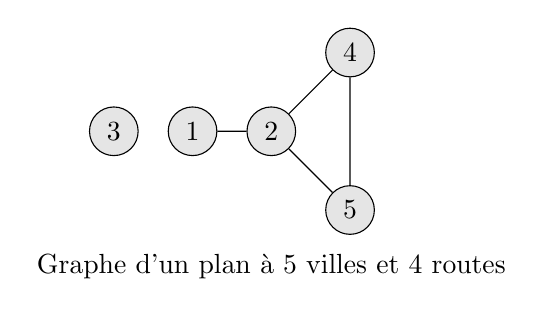
\begin{tikzpicture}[scale=1]
\tikzstyle{sommet}=[circle,draw,fill=gray!20]
\tikzstyle{arete}=[midway,fill=white]
\node[sommet] (S3) at (1,1) {3};
\node[sommet] (S1) at (2,1) {1};
\node[sommet] (S2) at (3,1) {2};
\node[sommet] (S4) at (4,2) {4};
\node[sommet] (S5) at (4,0) {5};
\draw (3,-1) node[above] {Graphe d'un plan à 5 villes et 4 routes} ;
\draw (S1) -- (S2) -- (S4)--(S5)--(S2) ; 
\end{tikzpicture}
\end{center}
\end{minipage}
\hfill
\begin{minipage}[c]{.45\linewidth}
\begin{lstlisting}
plan1= [[5,4] ,
         [1,2,None,None,None],
         [3,4,1,5,None],
         [0,None,None,None,None],
         [2,2,5,None,None],
         [2,4,2,None,None]]
\end{lstlisting}
\end{minipage}
 
\question{ Représenter sous forme de tableaux les deux plans suivants :}
\begin{center}
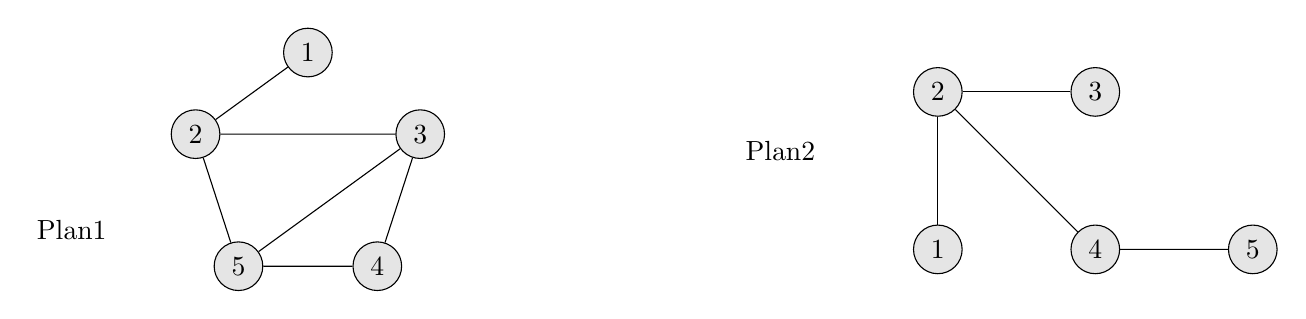
\begin{tikzpicture}[scale=1]
\tikzstyle{sommet}=[circle,draw,fill=gray!20]
\tikzstyle{arete}=[midway,fill=white]
\node[sommet] (A1) at ( 90:1.5) {1};
\node[sommet] (A2) at (162:1.5) {2};
\node[sommet] (A5) at (234:1.5) {5};
\node[sommet] (A4) at (306:1.5) {4};
\node[sommet] (A3) at ( 18:1.5) {3};
\draw (A1)--(A2)--(A3) -- (A4) -- (A5) --(A2);
\draw (A5)--(A3);
\draw (-3,-1) node[above] {Plan1} ;
\node[sommet] (B1) at (8,-1) {1};
\node[sommet] (B2) at (8,1) {2};
\node[sommet] (B3) at (10,1) {3};
\node[sommet] (B4) at (10,-1) {4};
\node[sommet] (B5) at (12,-1) {5};
\draw (6,0) node[above] {Plan2} ;
\draw (B1) -- (B2) -- (B3) ;
\draw (B2) -- (B4) -- (B5) ; 
\end{tikzpicture}
\end{center}


\question{ Écrire une fonction \texttt{creerPlanSansRoute(n:int)} qui crée, remplit et renvoie le tableau de tableaux correspondant au plan à $n$ villes n'ayant aucune route.}


\question{ Écrire une fonction \texttt{estVoisine(plan,x,y)} qui renvoie \texttt{True} si les villes \texttt{x} et \texttt{y} sont voisines dans le plan codé par le tableau de tableaux \texttt{plan} et renvoie \texttt{False} sinon.}


\question{Écrire une procédure \texttt{ajouteRoute(plan,x,y)} qui modifie le tableau de tableaux plan pour ajouter une route 
entre les villes \texttt{x} et \texttt{y} si elle n'était pas déjà présente et ne fait rien sinon. On prendra garde à bien mettre à jour
toutes les cases concernées dans le tableau de tableaux plan. Y a-t-il un risque de dépassement de la capacité des listes ?}

\question{Écrire une procédure \texttt{afficheToutesLesRoutes(plan)} qui affiche à l'écran la liste des routes du plan codé par le tableau de tableaux plan
où chaque route n'apparaît qu'une seule fois. Par exemple, pour le graphe codé par le tableau de tableaux de la présentation votre procédure pourra afficher :}
\begin{lstlisting}
`Ce plan contient 4 route(s) : (1-2) (2-4) (2-3) (4-5)`
\end{lstlisting}

\question{Quelle est la complexité de votre procédure ?}
